\question{13.4}{
    De Stichting voor Veilig Verkeer doet onderzoek naar de invloed van alcohol op het bloedalcoholgehalte (promillage).
    In een onderzoek onder tien mannen heeft men het promillage gemeten, twee uur na het begin van het drinken van vijf glazen bier.
    Tevens heeft men van deze tien personen het lichaamsgewicht gemeten.
    De gegevens staan in de tabel.
    \begin{center}
        \begin{tabular}{cc}
            \toprule
                {\bfseries Promillage} & {\bfseries Gewicht (in kg)} \\
            \cmidrule{1-1} \cmidrule{2-2}
                $1,06$ & $61$ \\
                $0,77$ & $82$ \\
                $0,72$ & $86$ \\
                $0,95$ & $70$ \\
                $0,65$ & $96$ \\
                $0,83$ & $80$ \\
                $0,99$ & $67$ \\
                $0,73$ & $90$ \\
                $0,84$ & $75$ \\
                $0,96$ & $73$ \\
            \bottomrule
        \end{tabular}
    \end{center}
    Een onderzoeker heeft het idee dat het gewicht van een persoon invloed heeft op het bloedalcoholgehalte en onderzoekt dit met regressie.
}
\begin{enumerate}[label=(\alph*)]
    \item Welke van de variabelen is de te verklaren variabele?
    \answer{
        De onderzoeker wil toetsen of het gewicht van een persoon invloed heeft op het promillage alcohol in het bloed van testpersonen.
        
        Dit houdt dus in dat de verklarende variabele $X$ het gewicht (in kg) is en de te verklaren variabele $Y$ het promillage alcohol in het bloed.
    }

    \item Stel de vergelijking van de regressielijn op.
    \answer{
        Bij enkelvoudige regressie is de regressielijn van de vorm $Y = a + b\cdot X$, waarbij we de regressieco\"effici\"enten $a$ en $b$ bepalen aan de hand van 
        \begin{align*}
            b &= \frac{\overline{xy} - \overline{x} \cdot \overline{y}}{\overline{x^2} - (\overline{x})^2} \\
            a &= \overline{y} - b \cdot \overline{x}
        \end{align*}
        We moeten dus een tabel construeren met de gemiddelde $\overline{x}$, $\overline{y}$, $\overline{xy}$ en $\overline{x^2}$.
        \begin{center}
            \begin{tabular}{cccc}
                \toprule
                    $x$ & $y$ & $xy$ & $x^2$ \\
                \midrule
                    $61$ & $1,06$ & $64,66$ & $3721$ \\
                    $82$ & $0,77$ & $63,14$ & $6724$ \\
                    $86$ & $0,72$ & $61,92$ & $7396$ \\
                    $70$ & $0,95$ & $66,5$  & $4900$ \\
                    $96$ & $0,65$ & $62,4$  & $9216$ \\
                    $80$ & $0,83$ & $66,4$  & $6400$ \\
                    $67$ & $0,99$ & $66,33$ & $4489$ \\
                    $90$ & $0,73$ & $65,7$  & $8100$ \\
                    $75$ & $0,84$ & $63$    & $5625$ \\
                    $73$ & $0,96$ & $70,08$ & $5329$ \\
                \midrule       			
                    $\overline{x} = 78$ & $\overline{y} = 0,85$ & $\overline{xy} = 65,013$ & $\overline{x^2} = 6190$ \\
                \bottomrule
            \end{tabular}
        \end{center}

        We hebben nu alle grootheden die benodigd zijn om de co\"effici\"enten van de regressielijn $Y = a + b \cdot X$ te kunnen bepalen:
        \begin{align*}
            b   &= \frac{\overline{xy} - \overline{x} \cdot \overline{y}}{\overline{x^2} - (\overline{x})^2} \\
                &= \frac{65,013 - 78 \cdot 0,85}{6190 - (78)^2} \\
                &= \frac{-1,287}{106} \approx -0,0121 \\
            a   &= \overline{y} - b \cdot \overline{x} \\
                &= 0,85 - ({-0,0121} \cdot 78) \\
                &\approx 1,7970.
        \end{align*}
        De formule van de regressielijn behorende bij deze steekproef is dus gelijk aan $Y = 1,7970-0,0121 \cdot X$.    
        
        \begin{center}
            \resizebox{0.9\textwidth}{!}{
                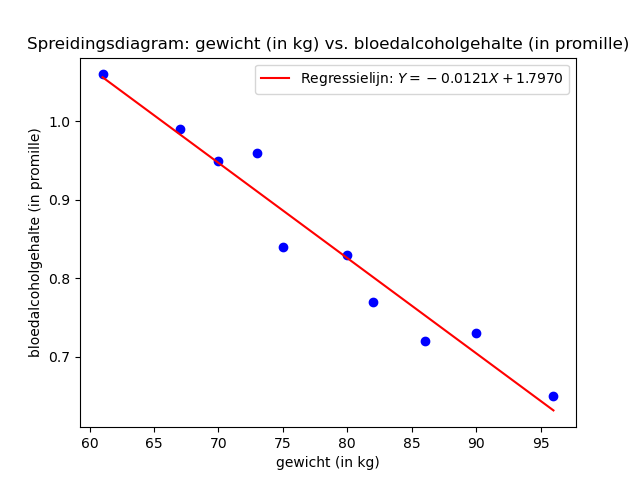
\includegraphics{opg13.4.png}
            }
        \end{center}
    }

    \item Bereken de correlatieco\"effici\"ent.
    \answer{
        De correlatieco\"effici\"ent $r(x, y)$ berekenen we op basis van de formule
        \[
            r(x, y) = \frac{\overline{x \cdot y} - \overline{x} \cdot \overline{y}}{\sqrt{(\overline{x}^2 - \overline{x^2})}}.
        \]
        Dat betekent dat we naast de bovenstaande tabel moeten uitbreiden met een kolom voor $y^2$:
        \begin{center}
            \begin{tabular}{ccccc}
                \toprule
                    $x$ & $y$ & $xy$ & $x^2$ & $y^2$ \\
                \midrule
                    $61$ & $1,06$ & $64,66$ & $3721$ & $1,1236$ \\
                    $82$ & $0,77$ & $63,14$ & $6724$ & $0,5929$ \\
                    $86$ & $0,72$ & $61,92$ & $7396$ & $0,5184$ \\
                    $70$ & $0,95$ & $66,5$ & $4900$ & $0,9025$ \\
                    $96$ & $0,65$ & $62,4$ & $9216$ & $0,4225$ \\
                    $80$ & $0,83$ & $66,4$ & $6400$ & $0,6889$ \\
                    $67$ & $0,99$ & $66,33$ & $4489$ & $0,9801$ \\
                    $90$ & $0,73$ & $65,7$ & $8100$ & $0,5329$ \\
                    $75$ & $0,84$ & $63$ & $5625$ & $0,7056$ \\
                    $73$ & $0,96$ & $70,08$ & $5329$ & $0,9216$ \\
                \midrule       			
                    $\overline{x} = 78$ & $\overline{y} = 0,85$ & $\overline{xy} = 65,013$ & $\overline{x^2} = 6190$ \\
                \bottomrule
            \end{tabular}
        \end{center}
        De correlatieco\"effici\"ent $r(x, y)$ is dus gelijk aan
        \begin{align*}
            r(x,y)  &= \frac{\overline{x \cdot y} - \overline{x} \cdot \overline{y}}{\sqrt{(\overline{x}^2 - \overline{x^2}) \cdot (\overline{y}^2 - \overline{y^2})}} \\
                    &= \frac{65,013 - 78 \cdot 0,85}{\sqrt{(78^2 - 6190) \cdot (0,85^2 - 0,739)}} \\
                    &= \frac{-1,287}{1,318} \\
                    &\approx -0,9761.
        \end{align*}
        {\itshape Sidenote: de correlatieco\"effici\"ent $r(x, y)$ ligt erg dicht in de buurt van $-1$, wat inhoudt dat er een sterke negatieve correlatie is tussen de variabelen bloedalcoholgehalte en gewicht.
        Naarmate iemand zwaarder is, zal het promillage in het bloed ook kleiner zijn bij consumptie van vijf glazen bier.}
            
    }

    \item Geef het voorspelde promillage (twee uur na het begin van het drinken van vijf glazen bier) voor een man van \SI{85}{\kilogram}.
    \answer{
        Een voorspelling voor het promillage twee uur na het begin van het drinken van vijf glazen bier bij een man die \SI{85}{\kilogram} weegt vinden we simpelweg door $X = 85$ in te vullen in de regressielijn.
        Dit geeft een voorspelde waarde van $Y = 1,7970 - 0,0121 \cdot 85 \approx 0,7650$. 
        
        Dat betekent dat bij een gewicht van \SI{85}{\kilogram}, het bloedalcoholgehalte naar verwachting gelijk is aan $0,7650$ promille.
    }

    \item Uit onderzoek is gebleken: het promillage ligt, twee uur na het begin van het drinken van zes glazen bier (bij mannen) \SI{20}{\percent} hoger dan na het drinken van vijf glazen.
    Stel de vergelijking van de regressielijn voor dit geval op.
    \answer{
        Merk op dat we nu alle waardes voor $y$ moeten vermenigvuldigen met $1,2$ (\SI{20}{\percent} meer dan bij vijf glazen bier).
        Dat betekent ook dat $\overline{y}$ en $\overline{xy}$ met een factor $1,2$ groter worden.

        De formule van de (nieuwe) regressielijn $Y = a_{\textrm{n}} + b_{\textrm{n}} \cdot X$ kunnen we opstellen met behulp van:
        \begin{align*}
            b_{\textrm{n}} &= \frac{\overline{xy}_{\textrm{n}} - \overline{x}_{\textrm{n}} \cdot \overline{y}_{\textrm{n}}}{\overline{x^2}_{\textrm{n}} - (\overline{x}_{\textrm{n}})^2} = \frac{(1,2 \cdot \overline{xy}) - \overline{x} \cdot (1,2 \cdot \overline{y})}{\overline{x^2} - (\overline{x})^2} = \frac{1,2 \cdot (\overline{xy} - \overline{x} \cdot \overline{y})}{\overline{x^2} - (\overline{x})^2} = 1,2 \cdot b\\
            a_{\textrm{n}} &= \overline{y}_{\textrm{n}} - b_{\textrm{n}} \cdot \overline{x}_{\textrm{n}} = 1,2 \cdot \overline{y} - 1,2 \cdot b \cdot \overline{x} = 1,2 \cdot (\overline{y} - b \cdot \overline{x}) = 1,2 \cdot a
        \end{align*}

        Dit betekent dus dat zowel het snijpunt $a$ met de $y$-as als de richtingsco\"effici\"ent $b$ van de regressielijn met een factor $1,2$ groter worden.
        
        De nieuwe regressielijn -- uitgaande van consumptie van zes glazen bier -- kan dus worden beschreven met
        \[
            Y = 1,2 \cdot a + 1,2 \cdot b \cdot X = 2,1564-0,0146 \cdot X.
        \]
    }   
\end{enumerate}